\documentclass[11pt]{article}

\usepackage[margin=1in]{geometry}
\usepackage[T1]{fontenc}
\usepackage{graphicx}
\usepackage{longtable}
\usepackage{booktabs}
\usepackage{array}
\usepackage{enumitem}
\usepackage{xcolor}
\usepackage{hyperref}
\usepackage{tikz}
\usepackage{float}
\usepackage{fancyhdr}
\usepackage{titlesec}
\usepackage{tcolorbox}
\usepackage{tabularx}
\usepackage{multirow}
\usepackage{caption}
\usepackage{listings}
\usepackage{makecell}
\usepackage{amssymb}
\usepackage{pifont}

\usetikzlibrary{shapes.geometric, arrows.meta, positioning, fit, backgrounds, calc, decorations.pathreplacing, shapes.multipart, matrix, shadows}

% ---------------------------------------------------------------------------
% Color Definitions
% ---------------------------------------------------------------------------
\definecolor{sectionblue}{RGB}{31,78,121}
\definecolor{isocolor}{RGB}{0,102,153}
\definecolor{conformcolor}{RGB}{60,179,113}
\definecolor{viewcolor}{RGB}{255,165,0}
\definecolor{flowcolor}{RGB}{100,100,100}
\definecolor{lightgray}{RGB}{245,245,245}
\definecolor{warningred}{RGB}{220,53,69}
\definecolor{successgreen}{RGB}{40,167,69}
\definecolor{infoblue}{RGB}{23,162,184}
\definecolor{stakeholdercolor}{RGB}{70,130,180}
\definecolor{concerncolor}{RGB}{186,85,211}
\definecolor{viewpointcolor}{RGB}{255,127,80}
\definecolor{modelcolor}{RGB}{144,238,144}
\definecolor{rationalecolor}{RGB}{255,182,193}

\hypersetup{
  colorlinks=true,
  linkcolor=sectionblue,
  urlcolor=sectionblue,
  citecolor=sectionblue
}

% ---------------------------------------------------------------------------
% Header and Footer
% ---------------------------------------------------------------------------
\pagestyle{fancy}
\fancyhf{}
\fancyhead[L]{\leftmark}
\fancyhead[R]{ISO/IEC/IEEE 42010 Conformance Guide}
\fancyfoot[C]{\thepage}
\renewcommand{\headrulewidth}{0.4pt}
\renewcommand{\footrulewidth}{0.4pt}

% ---------------------------------------------------------------------------
% Section Formatting
% ---------------------------------------------------------------------------
\titleformat{\section}
  {\normalfont\Large\bfseries\color{sectionblue}}{\thesection}{1em}{}
\titleformat{\subsection}
  {\normalfont\large\bfseries\color{sectionblue!80}}{\thesubsection}{1em}{}
\titleformat{\subsubsection}
  {\normalfont\normalsize\bfseries\color{sectionblue!60}}{\thesubsubsection}{1em}{}

% ---------------------------------------------------------------------------
% Custom Box Environments
% ---------------------------------------------------------------------------
\newtcolorbox{keypoint}{
    colback=blue!5,
    colframe=sectionblue,
    title=Key Point,
    fonttitle=\bfseries
}

\newtcolorbox{warning}{
    colback=red!5,
    colframe=warningred,
    title=Warning,
    fonttitle=\bfseries
}

\newtcolorbox{bestpractice}{
    colback=green!5,
    colframe=successgreen,
    title=Best Practice,
    fonttitle=\bfseries
}

\newtcolorbox{example}{
    colback=lightgray,
    colframe=flowcolor,
    title=Example,
    fonttitle=\bfseries
}

\newtcolorbox{definition}{
    colback=infoblue!10,
    colframe=infoblue,
    title=Definition,
    fonttitle=\bfseries
}

\newtcolorbox{isorequirement}[1][]{
    colback=isocolor!8,
    colframe=isocolor,
    title=#1,
    fonttitle=\bfseries,
    breakable
}

\newtcolorbox{conformancebox}[1][]{
    colback=conformcolor!10,
    colframe=conformcolor,
    title=#1,
    fonttitle=\bfseries
}

\newtcolorbox{questionbox}[1][]{
    colback=viewcolor!10,
    colframe=viewcolor,
    title=#1,
    fonttitle=\bfseries,
    breakable
}

\newtcolorbox{checklistbox}[1][]{
    colback=white,
    colframe=flowcolor,
    title=#1,
    fonttitle=\bfseries
}

\tcbuselibrary{listings}

% ---------------------------------------------------------------------------
% List Settings
% ---------------------------------------------------------------------------
\setlist[itemize]{leftmargin=*,topsep=3pt,itemsep=2pt,parsep=0pt}
\setlist[enumerate]{leftmargin=*,topsep=3pt,itemsep=2pt,parsep=0pt}

% ---------------------------------------------------------------------------
% Custom Column Types
% ---------------------------------------------------------------------------
\newcolumntype{L}[1]{>{\raggedright\arraybackslash}p{#1}}
\newcolumntype{C}[1]{>{\centering\arraybackslash}p{#1}}
\newcolumntype{R}[1]{>{\raggedleft\arraybackslash}p{#1}}

% ---------------------------------------------------------------------------
% Custom Commands
% ---------------------------------------------------------------------------
\newcommand{\AD}{architecture description}
\newcommand{\ADs}{architecture descriptions}
\newcommand{\isosection}[1]{\textcolor{isocolor}{\textbf{[\S#1]}}}
\newcommand{\conform}{\textcolor{successgreen}{\ding{51}}}
\newcommand{\nonconform}{\textcolor{warningred}{\ding{55}}}
\newcommand{\partaf}{\textcolor{viewcolor}{\ding{72}}}
\newcommand{\mandatory}{\textcolor{warningred}{\textbf{M}}}

% ---------------------------------------------------------------------------
% Title
% ---------------------------------------------------------------------------
\title{%
    \vspace{-1cm}
    \textbf{\Huge Software Architecture Documentation}\\[12pt]
    \Large Reviewing for Conformance to ISO/IEC/IEEE 42010\\[8pt]
    \large A Comprehensive Guide to Architecture Description\\
    Conformance Assessment and Certification
}
\author{%
    \textit{Architecture Documentation Series}\\[4pt]
    \small Based on ISO/IEC/IEEE 42010:2011 and Industry Best Practices
}
\date{\today}

\begin{document}
\maketitle
\thispagestyle{empty}

\vspace{0.5cm}

\begin{abstract}
\noindent
ISO/IEC/IEEE 42010:2011 establishes the international standard for architecture descriptions of systems and software. Conformance to this standard ensures that architecture documentation is complete, consistent, and useful to all stakeholders. This comprehensive guide provides detailed question sets, checklists, and assessment procedures for reviewing architecture descriptions against ISO/IEC/IEEE 42010 requirements. The document covers all conformance points including stakeholder identification, concern documentation, viewpoint specification, model kind definition, view construction, correspondence rules, and rationale capture. Whether conducting internal reviews, contract compliance assessments, or formal certification audits, this guide enables systematic and thorough conformance evaluation.
\end{abstract}

\vfill

\begin{center}
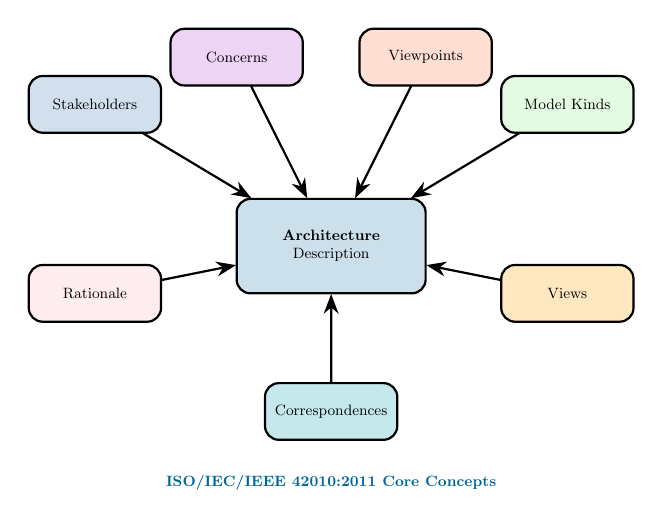
\begin{tikzpicture}[
    scale=0.6,
    transform shape,
    concept/.style={draw, thick, rounded corners=5pt, minimum width=2.8cm, minimum height=1.2cm, font=\small, align=center},
    arrow/.style={-{Stealth[length=2.5mm]}, thick}
]
    % Central AD
    \node[concept, fill=isocolor!20, minimum width=4cm, minimum height=2cm] (ad) at (0,0) {\textbf{Architecture}\\Description};
    
    % Core concepts
    \node[concept, fill=stakeholdercolor!25] (stake) at (-5,3) {Stakeholders};
    \node[concept, fill=concerncolor!25] (concern) at (-2,4) {Concerns};
    \node[concept, fill=viewpointcolor!25] (vp) at (2,4) {Viewpoints};
    \node[concept, fill=modelcolor!25] (model) at (5,3) {Model Kinds};
    \node[concept, fill=viewcolor!25] (view) at (5,-1) {Views};
    \node[concept, fill=rationalecolor!25] (rat) at (-5,-1) {Rationale};
    \node[concept, fill=infoblue!25] (corr) at (0,-3.5) {Correspondences};
    
    % Connections
    \draw[arrow] (stake) -- (ad);
    \draw[arrow] (concern) -- (ad);
    \draw[arrow] (vp) -- (ad);
    \draw[arrow] (model) -- (ad);
    \draw[arrow] (view) -- (ad);
    \draw[arrow] (rat) -- (ad);
    \draw[arrow] (corr) -- (ad);
    
    % ISO label
    \node[font=\bfseries\small, text=isocolor] at (0,-5) {ISO/IEC/IEEE 42010:2011 Core Concepts};
\end{tikzpicture}
\end{center}

\newpage
\tableofcontents
\newpage

%==============================================================================
\section{Introduction}
%==============================================================================

\subsection{Purpose of This Guide}

This guide provides comprehensive procedures for reviewing architecture descriptions (ADs) for conformance to ISO/IEC/IEEE 42010:2011, the international standard for architecture description of systems and software. Conformance review ensures that:

\begin{itemize}
    \item Architecture documentation meets international quality standards
    \item All required elements are present and properly documented
    \item Stakeholder needs are adequately addressed
    \item Documentation is consistent and usable
    \item Contractual or regulatory requirements are satisfied
\end{itemize}

\subsection{About ISO/IEC/IEEE 42010}

\begin{definition}
\textbf{ISO/IEC/IEEE 42010:2011} ``Systems and software engineering---Architecture description'' specifies the manner in which architecture descriptions of systems are organized and expressed. It defines the required content for an architecture description and establishes a conceptual foundation for architecture description.
\end{definition}

The standard applies to:
\begin{itemize}
    \item Software systems
    \item Systems containing software
    \item Enterprise and organizational architectures
    \item Product line architectures
    \item Reference architectures
\end{itemize}

\subsection{Conformance Requirements}

\begin{warning}
\textbf{All Requirements Are Mandatory}

ISO/IEC/IEEE 42010 contains no optional requirements or tailoring provisions. For an architecture description to claim conformance, it must satisfy \textbf{all} requirements specified in the standard. Partial conformance is not recognized.
\end{warning}

\subsection{Document Organization}

This guide is organized as follows:

\begin{itemize}
    \item \textbf{Section 2:} Overview of ISO/IEC/IEEE 42010 conceptual model and requirements
    \item \textbf{Section 3:} Detailed conformance requirements by category
    \item \textbf{Section 4:} Review question sets for conformance assessment
    \item \textbf{Section 5:} Conformance checklists and matrices
    \item \textbf{Section 6:} Common non-conformances and remediation
    \item \textbf{Section 7:} Review process guidelines
    \item \textbf{Appendices:} Templates, examples, and references
\end{itemize}

%==============================================================================
\section{ISO/IEC/IEEE 42010 Conceptual Model}
%==============================================================================

\subsection{Core Concepts}

The standard defines a conceptual model relating the key elements of architecture description. Understanding this model is essential for conformance review.

\begin{figure}[H]
\centering
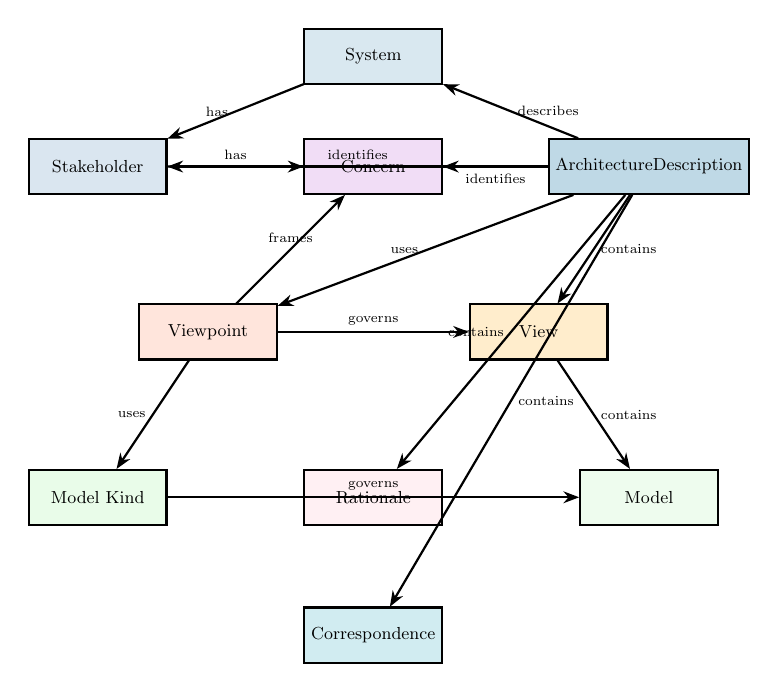
\begin{tikzpicture}[
    scale=0.7,
    transform shape,
    entity/.style={draw, thick, fill=white, minimum width=2.5cm, minimum height=1cm, font=\small},
    arrow/.style={-{Stealth[length=2mm]}, thick}
]
    % Entities
    \node[entity, fill=isocolor!15] (system) at (0,6) {System};
    \node[entity, fill=stakeholdercolor!20] (stakeholder) at (-5,4) {Stakeholder};
    \node[entity, fill=concerncolor!20] (concern) at (0,4) {Concern};
    \node[entity, fill=isocolor!25] (ad) at (5,4) {Architecture\\Description};
    \node[entity, fill=viewpointcolor!20] (viewpoint) at (-3,1) {Viewpoint};
    \node[entity, fill=viewcolor!20] (view) at (3,1) {View};
    \node[entity, fill=modelcolor!20] (modelkind) at (-5,-2) {Model Kind};
    \node[entity, fill=modelcolor!15] (model) at (5,-2) {Model};
    \node[entity, fill=rationalecolor!20] (rationale) at (0,-2) {Rationale};
    \node[entity, fill=infoblue!20] (corr) at (0,-4.5) {Correspondence};
    
    % Relationships
    \draw[arrow] (system) -- node[left, font=\scriptsize] {has} (stakeholder);
    \draw[arrow] (stakeholder) -- node[above, font=\scriptsize] {has} (concern);
    \draw[arrow] (ad) -- node[right, font=\scriptsize] {describes} (system);
    \draw[arrow] (ad) -- node[above, font=\scriptsize] {identifies} (stakeholder);
    \draw[arrow] (ad) -- node[below, font=\scriptsize] {identifies} (concern);
    \draw[arrow] (viewpoint) -- node[above, font=\scriptsize] {frames} (concern);
    \draw[arrow] (viewpoint) -- node[above, font=\scriptsize] {governs} (view);
    \draw[arrow] (ad) -- node[left, font=\scriptsize] {uses} (viewpoint);
    \draw[arrow] (ad) -- node[right, font=\scriptsize] {contains} (view);
    \draw[arrow] (viewpoint) -- node[left, font=\scriptsize] {uses} (modelkind);
    \draw[arrow] (view) -- node[right, font=\scriptsize] {contains} (model);
    \draw[arrow] (modelkind) -- node[above, font=\scriptsize] {governs} (model);
    \draw[arrow] (ad) -- node[left, font=\scriptsize] {contains} (rationale);
    \draw[arrow] (ad) -- node[right, font=\scriptsize] {contains} (corr);
\end{tikzpicture}
\caption{ISO/IEC/IEEE 42010 Conceptual Model (Simplified)}
\end{figure}

\subsection{Key Definitions}

\begin{longtable}{@{}L{3cm} L{9.5cm}@{}}
\caption{ISO/IEC/IEEE 42010 Key Terms} \\
\toprule
\textbf{Term} & \textbf{Definition} \\
\midrule
\endfirsthead
\toprule
\textbf{Term} & \textbf{Definition} \\
\midrule
\endhead
\bottomrule
\endlastfoot
Architecture & Fundamental concepts or properties of a system in its environment embodied in its elements, relationships, and in the principles of its design and evolution \\
Architecture Description & Work product used to express an architecture \\
Stakeholder & Individual, team, organization, or classes thereof, having an interest in a system \\
Concern & Interest in a system relevant to one or more of its stakeholders \\
Viewpoint & Work product establishing the conventions for the construction, interpretation, and use of architecture views to frame specific system concerns \\
View & Work product expressing the architecture of a system from the perspective of specific system concerns \\
Model Kind & Conventions for a type of modeling \\
Model & An artifact that expresses information about a system from a particular perspective as defined by its model kind \\
Correspondence & A relation between AD elements; used to express and enforce architecture relations \\
Correspondence Rule & A rule governing correspondences; defines constraints on AD elements \\
Architecture Framework & Conventions, principles, and practices for the description of architectures established within a specific domain or stakeholder community \\
Rationale & Explanation or justification of decisions made \\
\end{longtable}

\subsection{Conformance Scope}

\begin{keypoint}
\textbf{What Must Conform}

ISO/IEC/IEEE 42010 specifies requirements for \textbf{architecture descriptions}, not for architectures themselves. The standard does not prescribe how to architect systems; it specifies how to document architectures. Conformance assessment evaluates the documentation, not the quality of architectural decisions.
\end{keypoint}

%==============================================================================
\section{Detailed Conformance Requirements}
%==============================================================================

This section presents the conformance requirements organized by category, with references to the relevant standard sections.

\subsection{Architecture Description Identification \isosection{5.2}}

\begin{isorequirement}[AD Identification Requirements]
An architecture description shall include information to identify it, including:

\begin{enumerate}
    \item Date of issue and status
    \item Issuing organization
    \item Change history
    \item Summary
    \item Scope
    \item Context
    \item Glossary of terms
    \item References
\end{enumerate}
\end{isorequirement}

\begin{longtable}{@{}L{3cm} L{5cm} L{4.5cm}@{}}
\caption{AD Identification Elements} \\
\toprule
\textbf{Element} & \textbf{Description} & \textbf{Verification} \\
\midrule
\endfirsthead
\bottomrule
\endlastfoot
Date of Issue & Publication or release date & Check document header/metadata \\
Status & Draft, review, approved, etc. & Check document status indicator \\
Issuing Organization & Organization responsible for the AD & Check authorship information \\
Change History & Record of changes across versions & Check change log/revision history \\
Summary & Brief overview of the AD & Check executive summary section \\
Scope & What the AD covers and excludes & Check scope statement \\
Context & Environmental and background information & Check context section \\
Glossary & Definitions of terms used & Check glossary/definitions section \\
References & External documents referenced & Check references/bibliography \\
\end{longtable}

\subsection{Stakeholder and Concern Identification \isosection{5.3}}

\begin{isorequirement}[Stakeholder and Concern Requirements]
An architecture description shall identify:

\begin{enumerate}
    \item The stakeholders having concerns about the system
    \item The concerns considered fundamental to the architecture
\end{enumerate}

Every identified concern shall be framed by at least one viewpoint used in the AD.

The AD shall consider at minimum these stakeholder classes:
\begin{itemize}[nosep]
    \item Users of the system
    \item Operators of the system
    \item Acquirers of the system
    \item Owners of the system
    \item Suppliers of the system
    \item Developers of the system
    \item Builders of the system
    \item Maintainers of the system
\end{itemize}

The AD shall consider at minimum these concerns:
\begin{itemize}[nosep]
    \item The purposes of the system
    \item The suitability of the architecture for achieving system purposes
    \item The feasibility of constructing and deploying the system
    \item The potential risks and impacts of the system
    \item Maintainability and evolvability of the system
\end{itemize}
\end{isorequirement}

\subsection{Viewpoint Specification \isosection{5.4}}

\begin{isorequirement}[Viewpoint Requirements]
For each viewpoint used in an AD, the AD shall include or reference a viewpoint specification that includes:

\begin{enumerate}
    \item Viewpoint name
    \item Stakeholders addressed by the viewpoint
    \item Concerns framed by the viewpoint
    \item Model kinds used in the viewpoint
    \item For each model kind:
    \begin{itemize}[nosep]
        \item Conventions: languages, notations, modeling techniques
        \item Operations on models (if any)
    \end{itemize}
    \item Sources for the viewpoint (if any)
\end{enumerate}
\end{isorequirement}

\begin{figure}[H]
\centering
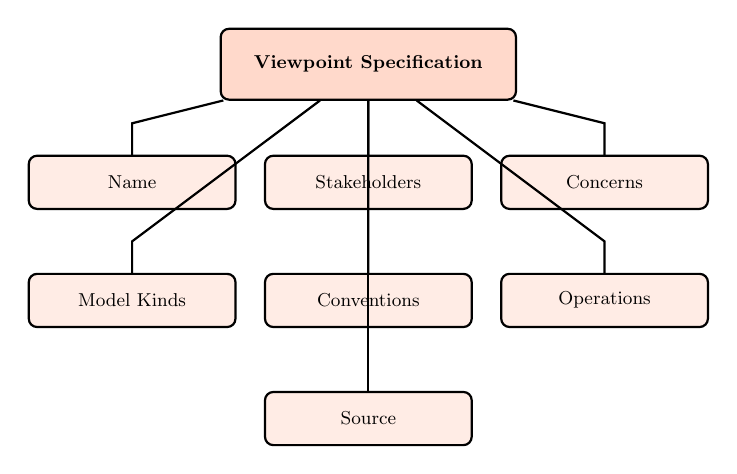
\begin{tikzpicture}[
    scale=0.75,
    transform shape,
    box/.style={draw, thick, fill=viewpointcolor!15, minimum width=3.5cm, minimum height=0.9cm, rounded corners=3pt, font=\small},
    arrow/.style={-{Stealth[length=2mm]}, thick}
]
    % Viewpoint specification structure
    \node[box, fill=viewpointcolor!30, minimum width=5cm, minimum height=1.2cm] (vp) at (0,4) {\textbf{Viewpoint Specification}};
    
    \node[box] (name) at (-4,2) {Name};
    \node[box] (stake) at (0,2) {Stakeholders};
    \node[box] (concern) at (4,2) {Concerns};
    \node[box] (mk) at (-4,0) {Model Kinds};
    \node[box] (conv) at (0,0) {Conventions};
    \node[box] (ops) at (4,0) {Operations};
    \node[box] (src) at (0,-2) {Source};
    
    % Connections
    \draw[thick] (vp) -- (-4,3) -- (name);
    \draw[thick] (vp) -- (0,3) -- (stake);
    \draw[thick] (vp) -- (4,3) -- (concern);
    \draw[thick] (vp) -- (-4,1) -- (mk);
    \draw[thick] (vp) -- (0,1) -- (conv);
    \draw[thick] (vp) -- (4,1) -- (ops);
    \draw[thick] (vp) -- (src);
\end{tikzpicture}
\caption{Viewpoint Specification Elements}
\end{figure}

\subsection{Model Kind Specification \isosection{5.5}}

\begin{isorequirement}[Model Kind Requirements]
Each model kind used in an AD shall specify:

\begin{enumerate}
    \item The conventions for models of that kind, including:
    \begin{itemize}[nosep]
        \item Language, notation, or modeling technique used
        \item How models of this kind are to be constructed
        \item How models of this kind are to be interpreted
    \end{itemize}
    \item Operations defined on models of that kind (if applicable)
    \item Any correspondence rules associated with the model kind
\end{enumerate}
\end{isorequirement}

\subsection{View and Model Requirements \isosection{5.6}}

\begin{isorequirement}[View Requirements]
For each viewpoint selected for use in an AD:

\begin{enumerate}
    \item The AD shall contain exactly one view governed by that viewpoint
    \item Each view shall adhere to the conventions of its governing viewpoint
    \item Each view shall include one or more models
    \item Each model shall adhere to the conventions of its governing model kind
\end{enumerate}
\end{isorequirement}

\subsection{Correspondence and Correspondence Rules \isosection{5.7}}

\begin{isorequirement}[Correspondence Requirements]
An architecture description shall:

\begin{enumerate}
    \item Record any correspondences between its AD elements
    \item Record any correspondence rules, whether from:
    \begin{itemize}[nosep]
        \item Architecture framework requirements
        \item Viewpoint specifications
        \item Model kind specifications
        \item AD-specific rules
    \end{itemize}
    \item For each correspondence rule, identify at least one correspondence satisfying that rule, or document known inconsistencies
\end{enumerate}
\end{isorequirement}

\begin{example}
\textbf{Correspondence Rule Example}

\textbf{Rule:} Every module in the Module Decomposition View shall map to at least one runtime component in the Component-and-Connector View.

\textbf{Satisfying Correspondences:}
\begin{itemize}[nosep]
    \item OrderModule $\rightarrow$ OrderService
    \item PaymentModule $\rightarrow$ PaymentService
    \item UserModule $\rightarrow$ UserService, AuthService
\end{itemize}
\end{example}

\subsection{Rationale Requirements \isosection{5.8}}

\begin{isorequirement}[Rationale Requirements]
An architecture description shall record the rationale for:

\begin{enumerate}
    \item Selection of viewpoints used
    \item Selection of model kinds used
    \item Correspondence rules specified
    \item Decisions captured in views and models
\end{enumerate}

Rationale may be recorded within views, as separate rationale items, or both.
\end{isorequirement}

\subsection{Architecture Framework Usage \isosection{6}}

\begin{isorequirement}[Architecture Framework Requirements]
When an AD uses an architecture framework:

\begin{enumerate}
    \item The AD shall cite the framework
    \item The AD shall use the viewpoints defined by the framework (or justify exceptions)
    \item The AD shall apply correspondence rules defined by the framework
    \item The AD shall conform to any additional requirements of the framework
\end{enumerate}
\end{isorequirement}

%==============================================================================
\section{Review Question Sets}
%==============================================================================

\subsection{Question Set Overview}

\begin{keypoint}
\textbf{Review Purpose}

These question sets assess conformance of an architecture description to ISO/IEC/IEEE 42010 requirements. The questions are organized by conformance area and respondent role. Positive answers with documented evidence indicate conformance.
\end{keypoint}

\subsection{Questions for Architects}

\begin{questionbox}[Architecture Description Identification Questions]

\textbf{Conformance Area:} AD Identification \isosection{5.2}

\begin{enumerate}
    \item Does the AD include a clearly visible date of issue?
    \begin{itemize}[nosep]
        \item Where is the date located?
        \item Is the date format unambiguous (e.g., ISO 8601)?
    \end{itemize}
    
    \item Does the AD include a status indicator (draft, review, approved, etc.)?
    \begin{itemize}[nosep]
        \item What is the current status?
        \item Who authorizes status changes?
    \end{itemize}
    
    \item Does the AD identify the issuing organization?
    \begin{itemize}[nosep]
        \item Is the responsible organization clearly named?
        \item Are author(s) identified?
    \end{itemize}
    
    \item Does the AD include a change history?
    \begin{itemize}[nosep]
        \item Does the history include version numbers?
        \item Are changes summarized for each version?
        \item Are change authors and dates recorded?
    \end{itemize}
    
    \item Does the AD include a summary?
    \begin{itemize}[nosep]
        \item Does the summary provide a high-level overview?
        \item Can a reader quickly understand the AD's purpose?
    \end{itemize}
    
    \item Does the AD define its scope?
    \begin{itemize}[nosep]
        \item Is the system being described clearly identified?
        \item Are scope boundaries explicit (what's in and out)?
    \end{itemize}
    
    \item Does the AD establish context?
    \begin{itemize}[nosep]
        \item Is the system's environment described?
        \item Are external entities and interfaces identified?
    \end{itemize}
    
    \item Does the AD include a glossary?
    \begin{itemize}[nosep]
        \item Are domain-specific terms defined?
        \item Are architecture-specific terms defined?
        \item Is terminology used consistently throughout?
    \end{itemize}
    
    \item Does the AD include references?
    \begin{itemize}[nosep]
        \item Are external documents properly cited?
        \item Are referenced documents accessible to readers?
    \end{itemize}
\end{enumerate}
\end{questionbox}

\begin{questionbox}[Stakeholder and Concern Questions]

\textbf{Conformance Area:} Stakeholders and Concerns \isosection{5.3}

\begin{enumerate}[resume]
    \item Are stakeholders explicitly identified?
    \begin{itemize}[nosep]
        \item Where in the AD is the stakeholder list?
        \item Are stakeholders identified by role or by name?
    \end{itemize}
    
    \item Does the AD consider the required stakeholder classes?
    \begin{itemize}[nosep]
        \item Users? (Yes/No/N/A with justification)
        \item Operators?
        \item Acquirers?
        \item Owners?
        \item Suppliers?
        \item Developers?
        \item Builders?
        \item Maintainers?
    \end{itemize}
    
    \item Are concerns explicitly identified?
    \begin{itemize}[nosep]
        \item Where in the AD is the concern list?
        \item Are concerns traced to stakeholders?
    \end{itemize}
    
    \item Does the AD consider the required concerns?
    \begin{itemize}[nosep]
        \item System purposes?
        \item Architectural suitability?
        \item Construction feasibility?
        \item Deployment feasibility?
        \item Risks and impacts?
        \item Maintainability?
        \item Evolvability?
    \end{itemize}
    
    \item Is every identified concern framed by at least one viewpoint?
    \begin{itemize}[nosep]
        \item Show the concern-to-viewpoint mapping
        \item Identify any concerns not covered
    \end{itemize}
\end{enumerate}
\end{questionbox}

\begin{questionbox}[Viewpoint Specification Questions]

\textbf{Conformance Area:} Viewpoints \isosection{5.4}

\begin{enumerate}[resume]
    \item For each viewpoint used, does the AD include or reference a viewpoint specification?
    \begin{itemize}[nosep]
        \item List all viewpoints used
        \item For each, indicate: included in AD / referenced externally
    \end{itemize}
    
    \item Does each viewpoint specification include a name?
    
    \item Does each viewpoint specification identify the stakeholders it addresses?
    
    \item Does each viewpoint specification identify the concerns it frames?
    
    \item Does each viewpoint specification identify model kinds used?
    
    \item For each model kind, are conventions specified?
    \begin{itemize}[nosep]
        \item Languages or notations?
        \item Modeling techniques?
        \item Construction guidance?
        \item Interpretation guidance?
    \end{itemize}
    
    \item Are operations on models specified (if applicable)?
    
    \item Are viewpoint sources cited (if applicable)?
\end{enumerate}
\end{questionbox}

\begin{questionbox}[View and Model Questions]

\textbf{Conformance Area:} Views and Models \isosection{5.6}

\begin{enumerate}[resume]
    \item For each viewpoint, does the AD contain exactly one corresponding view?
    \begin{itemize}[nosep]
        \item List viewpoint-to-view mapping
        \item Identify any viewpoints without views
        \item Identify any views without viewpoints
    \end{itemize}
    
    \item Does each view adhere to its governing viewpoint's conventions?
    
    \item Does each view contain at least one model?
    
    \item Does each model adhere to its governing model kind's conventions?
    
    \item Is the notation used in each model clearly documented or evident?
    
    \item Are the views complete relative to the concerns they address?
\end{enumerate}
\end{questionbox}

\begin{questionbox}[Correspondence Questions]

\textbf{Conformance Area:} Correspondences \isosection{5.7}

\begin{enumerate}[resume]
    \item Does the AD identify correspondence rules?
    \begin{itemize}[nosep]
        \item From architecture framework?
        \item From viewpoint specifications?
        \item From model kind specifications?
        \item AD-specific rules?
    \end{itemize}
    
    \item For each correspondence rule, is there at least one satisfying correspondence?
    
    \item Are any known inconsistencies documented?
    \begin{itemize}[nosep]
        \item What is the inconsistency?
        \item What is the impact?
        \item What is the resolution plan?
    \end{itemize}
    
    \item Does the AD record correspondences between AD elements?
    \begin{itemize}[nosep]
        \item Between views?
        \item Between models?
        \item Between other AD elements?
    \end{itemize}
\end{enumerate}
\end{questionbox}

\begin{questionbox}[Rationale Questions]

\textbf{Conformance Area:} Rationale \isosection{5.8}

\begin{enumerate}[resume]
    \item Is rationale provided for viewpoint selection?
    \begin{itemize}[nosep]
        \item Why were these viewpoints chosen?
        \item Why were other viewpoints not used?
    \end{itemize}
    
    \item Is rationale provided for model kind selection?
    
    \item Is rationale provided for correspondence rules?
    
    \item Is rationale provided for key architectural decisions?
    \begin{itemize}[nosep]
        \item Are major decisions identified?
        \item Are alternatives considered documented?
        \item Are selection criteria documented?
    \end{itemize}
    
    \item Is the rationale accessible and understandable?
    \begin{itemize}[nosep]
        \item Can readers find rationale for specific decisions?
        \item Is the rationale sufficient for understanding?
    \end{itemize}
\end{enumerate}
\end{questionbox}

\subsection{Questions for Acquirers and Analysts}

\begin{questionbox}[Acquirer/Analyst Assessment Questions]

\textbf{Respondents:} Acquirers, Architecture Analysts, Reviewers

\begin{enumerate}
    \item \textbf{Stakeholder Completeness:} Is the set of identified stakeholders complete?
    \begin{itemize}[nosep]
        \item Are all relevant parties represented?
        \item Are any stakeholders missing?
        \item Would the AD serve all identified stakeholders?
    \end{itemize}
    
    \item \textbf{Concern Completeness:} Is the set of identified concerns complete?
    \begin{itemize}[nosep]
        \item Are all architecturally significant concerns captured?
        \item Are concerns appropriately prioritized?
        \item Are any concerns missing?
    \end{itemize}
    
    \item \textbf{Viewpoint Completeness:} Is the set of viewpoints complete and minimal?
    \begin{itemize}[nosep]
        \item Do the viewpoints address all concerns?
        \item Are there redundant viewpoints?
        \item Are any essential viewpoints missing?
    \end{itemize}
    
    \item \textbf{View Quality:} Are the views complete and communicative?
    \begin{itemize}[nosep]
        \item Do views communicate key decisions?
        \item Is the level of detail appropriate?
        \item Can stakeholders understand the views?
    \end{itemize}
    
    \item \textbf{Correspondence Appropriateness:} Are correspondence rules appropriate?
    \begin{itemize}[nosep]
        \item Do rules capture important relationships?
        \item Are rules verifiable?
        \item Are correspondences documented?
    \end{itemize}
    
    \item \textbf{Rationale Sufficiency:} Does the rationale support understanding?
    \begin{itemize}[nosep]
        \item Can reviewers understand why decisions were made?
        \item Is rationale sufficient for analysis?
        \item Would rationale help future maintainers?
    \end{itemize}
    
    \item \textbf{Framework Compliance:} If a framework is used, is compliance achieved?
    \begin{itemize}[nosep]
        \item Are framework viewpoints used?
        \item Are framework correspondence rules applied?
        \item Are deviations justified?
    \end{itemize}
    
    \item \textbf{Contractual Compliance:} Does the AD meet contractual requirements?
    \begin{itemize}[nosep]
        \item Are contract-specified views present?
        \item Are contract-specified contents present?
        \item Are delivery requirements met?
    \end{itemize}
\end{enumerate}
\end{questionbox}

%==============================================================================
\section{Conformance Checklists and Matrices}
%==============================================================================

\subsection{Master Conformance Checklist}

\begin{checklistbox}[ISO/IEC/IEEE 42010 Conformance Checklist]

\textbf{AD Identification} \isosection{5.2}
\begin{itemize}[leftmargin=1.5cm]
    \item[$\square$] Date of issue included
    \item[$\square$] Status indicated
    \item[$\square$] Issuing organization identified
    \item[$\square$] Change history present
    \item[$\square$] Summary provided
    \item[$\square$] Scope defined
    \item[$\square$] Context established
    \item[$\square$] Glossary included
    \item[$\square$] References listed
\end{itemize}

\textbf{Stakeholders and Concerns} \isosection{5.3}
\begin{itemize}[leftmargin=1.5cm]
    \item[$\square$] Stakeholders identified
    \item[$\square$] Required stakeholder classes considered
    \item[$\square$] Concerns identified
    \item[$\square$] Required concerns considered
    \item[$\square$] Every concern framed by at least one viewpoint
\end{itemize}

\textbf{Viewpoints} \isosection{5.4}
\begin{itemize}[leftmargin=1.5cm]
    \item[$\square$] Viewpoint specifications included or referenced
    \item[$\square$] Viewpoint names specified
    \item[$\square$] Viewpoint stakeholders specified
    \item[$\square$] Viewpoint concerns specified
    \item[$\square$] Model kinds specified
    \item[$\square$] Model kind conventions specified
    \item[$\square$] Operations specified (if applicable)
    \item[$\square$] Sources cited (if applicable)
\end{itemize}

\textbf{Views and Models} \isosection{5.6}
\begin{itemize}[leftmargin=1.5cm]
    \item[$\square$] One view per viewpoint
    \item[$\square$] Views conform to viewpoint conventions
    \item[$\square$] Each view contains at least one model
    \item[$\square$] Models conform to model kind conventions
\end{itemize}

\textbf{Correspondences} \isosection{5.7}
\begin{itemize}[leftmargin=1.5cm]
    \item[$\square$] Correspondence rules identified
    \item[$\square$] Correspondences satisfy rules
    \item[$\square$] Known inconsistencies documented
\end{itemize}

\textbf{Rationale} \isosection{5.8}
\begin{itemize}[leftmargin=1.5cm]
    \item[$\square$] Viewpoint selection rationale
    \item[$\square$] Model kind selection rationale
    \item[$\square$] Correspondence rule rationale
    \item[$\square$] Decision rationale in views
\end{itemize}

\textbf{Architecture Framework} \isosection{6} (if applicable)
\begin{itemize}[leftmargin=1.5cm]
    \item[$\square$] Framework cited
    \item[$\square$] Framework viewpoints used
    \item[$\square$] Framework correspondence rules applied
    \item[$\square$] Deviations justified
\end{itemize}
\end{checklistbox}

\subsection{Conformance Assessment Matrix}

\begin{longtable}{@{}L{4cm} C{1.2cm} C{1.2cm} C{1.2cm} L{4.5cm}@{}}
\caption{Conformance Assessment Matrix Template} \\
\toprule
\textbf{Requirement} & \textbf{Conform} & \textbf{Non-Conform} & \textbf{N/A} & \textbf{Evidence / Notes} \\
\midrule
\endfirsthead
\toprule
\textbf{Requirement} & \textbf{Conform} & \textbf{Non-Conform} & \textbf{N/A} & \textbf{Evidence / Notes} \\
\midrule
\endhead
\bottomrule
\endlastfoot
\multicolumn{5}{l}{\textbf{AD Identification \isosection{5.2}}} \\
\quad Date of issue & $\square$ & $\square$ & $\square$ & \\
\quad Status & $\square$ & $\square$ & $\square$ & \\
\quad Issuing organization & $\square$ & $\square$ & $\square$ & \\
\quad Change history & $\square$ & $\square$ & $\square$ & \\
\quad Summary & $\square$ & $\square$ & $\square$ & \\
\quad Scope & $\square$ & $\square$ & $\square$ & \\
\quad Context & $\square$ & $\square$ & $\square$ & \\
\quad Glossary & $\square$ & $\square$ & $\square$ & \\
\quad References & $\square$ & $\square$ & $\square$ & \\
\midrule
\multicolumn{5}{l}{\textbf{Stakeholders and Concerns \isosection{5.3}}} \\
\quad Stakeholders identified & $\square$ & $\square$ & $\square$ & \\
\quad Required classes considered & $\square$ & $\square$ & $\square$ & \\
\quad Concerns identified & $\square$ & $\square$ & $\square$ & \\
\quad Required concerns considered & $\square$ & $\square$ & $\square$ & \\
\quad Concerns framed by viewpoints & $\square$ & $\square$ & $\square$ & \\
\midrule
\multicolumn{5}{l}{\textbf{Viewpoints \isosection{5.4}}} \\
\quad Specifications present & $\square$ & $\square$ & $\square$ & \\
\quad Names specified & $\square$ & $\square$ & $\square$ & \\
\quad Stakeholders specified & $\square$ & $\square$ & $\square$ & \\
\quad Concerns specified & $\square$ & $\square$ & $\square$ & \\
\quad Model kinds specified & $\square$ & $\square$ & $\square$ & \\
\quad Conventions specified & $\square$ & $\square$ & $\square$ & \\
\midrule
\multicolumn{5}{l}{\textbf{Views and Models \isosection{5.6}}} \\
\quad One view per viewpoint & $\square$ & $\square$ & $\square$ & \\
\quad Views conform to viewpoints & $\square$ & $\square$ & $\square$ & \\
\quad Models in each view & $\square$ & $\square$ & $\square$ & \\
\quad Models conform to kinds & $\square$ & $\square$ & $\square$ & \\
\midrule
\multicolumn{5}{l}{\textbf{Correspondences \isosection{5.7}}} \\
\quad Rules identified & $\square$ & $\square$ & $\square$ & \\
\quad Correspondences satisfy rules & $\square$ & $\square$ & $\square$ & \\
\quad Inconsistencies documented & $\square$ & $\square$ & $\square$ & \\
\midrule
\multicolumn{5}{l}{\textbf{Rationale \isosection{5.8}}} \\
\quad Viewpoint rationale & $\square$ & $\square$ & $\square$ & \\
\quad Model kind rationale & $\square$ & $\square$ & $\square$ & \\
\quad Correspondence rationale & $\square$ & $\square$ & $\square$ & \\
\quad Decision rationale & $\square$ & $\square$ & $\square$ & \\
\end{longtable}

\subsection{Stakeholder-Concern-Viewpoint Traceability}

\begin{longtable}{@{}L{2.5cm} L{3cm} L{3cm} C{1.5cm} C{1.5cm}@{}}
\caption{Stakeholder-Concern-Viewpoint Traceability} \\
\toprule
\textbf{Stakeholder} & \textbf{Concern} & \textbf{Viewpoint} & \textbf{Framed} & \textbf{View Present} \\
\midrule
\endfirsthead
\bottomrule
\endlastfoot
Developer & Code structure & Module & \conform & \conform \\
Developer & Dependencies & Uses & \conform & \conform \\
Operator & Deployment & Deployment & \conform & \conform \\
Operator & Runtime behavior & C\&C & \conform & \conform \\
Acquirer & System scope & Context & \conform & \conform \\
Acquirer & Decisions & Rationale & \conform & \conform \\
Maintainer & Modifiability & Module & \conform & \conform \\
User & Functionality & Functional & \conform & \partaf \\
\multicolumn{5}{l}{\scriptsize \conform = Complete \quad \partaf = Partial \quad \nonconform = Missing} \\
\end{longtable}

%==============================================================================
\section{Common Non-Conformances and Remediation}
%==============================================================================

\subsection{Non-Conformance Categories}

\begin{longtable}{@{}L{3cm} L{4.5cm} L{5cm}@{}}
\caption{Common Non-Conformances} \\
\toprule
\textbf{Category} & \textbf{Typical Issue} & \textbf{Remediation} \\
\midrule
\endfirsthead
\toprule
\textbf{Category} & \textbf{Typical Issue} & \textbf{Remediation} \\
\midrule
\endhead
\bottomrule
\endlastfoot
\multicolumn{3}{l}{\textbf{AD Identification}} \\
Missing metadata & No date, status, or version & Add document control section \\
No change history & Changes not tracked & Establish version control; add change log \\
Missing glossary & Terms undefined & Create glossary of domain and architecture terms \\
\midrule
\multicolumn{3}{l}{\textbf{Stakeholders and Concerns}} \\
Implicit stakeholders & Stakeholders not listed & Create explicit stakeholder registry \\
Missing classes & Required classes not considered & Review against standard's list; justify exclusion \\
Concerns not traced & Concerns not linked to stakeholders & Create stakeholder-concern mapping \\
Unframed concerns & Concerns without viewpoints & Add viewpoints or extend existing ones \\
\midrule
\multicolumn{3}{l}{\textbf{Viewpoints}} \\
Missing specifications & Viewpoints used but not defined & Create or reference viewpoint specifications \\
Incomplete specifications & Required elements missing & Complete specification with all required elements \\
No model kinds & Model kinds not specified & Define model kinds for each viewpoint \\
Missing conventions & Languages/notations not specified & Document notation and modeling conventions \\
\midrule
\multicolumn{3}{l}{\textbf{Views and Models}} \\
View-viewpoint mismatch & Views don't match viewpoints & Align views to viewpoint specifications \\
Empty views & Views without models & Add required models to each view \\
Convention violations & Models don't follow conventions & Revise models to conform to model kind specs \\
\midrule
\multicolumn{3}{l}{\textbf{Correspondences}} \\
No correspondence rules & Rules not documented & Identify and document correspondence rules \\
Unsatisfied rules & Rules without correspondences & Create correspondences or document inconsistencies \\
Hidden inconsistencies & Inconsistencies not documented & Document known inconsistencies with impact \\
\midrule
\multicolumn{3}{l}{\textbf{Rationale}} \\
Missing rationale & No decision justification & Add rationale for viewpoints, models, decisions \\
Incomplete rationale & Some decisions unjustified & Identify gaps; add missing rationale \\
Inaccessible rationale & Rationale hard to find & Organize rationale; add cross-references \\
\end{longtable}

\subsection{Severity Classification}

\begin{longtable}{@{}L{2cm} L{4cm} L{6.5cm}@{}}
\caption{Non-Conformance Severity Levels} \\
\toprule
\textbf{Severity} & \textbf{Definition} & \textbf{Examples} \\
\midrule
\endfirsthead
\bottomrule
\endlastfoot
\textcolor{warningred}{\textbf{Critical}} & Prevents conformance claim; must be resolved & Missing viewpoint specifications; no stakeholder identification; views without models \\
\textcolor{viewcolor}{\textbf{Major}} & Significant gap; high priority for resolution & Incomplete viewpoint specs; missing required concerns; inadequate rationale \\
\textcolor{flowcolor}{\textbf{Minor}} & Partial gap; should be resolved & Minor metadata missing; incomplete glossary; some conventions unstated \\
\end{longtable}

%==============================================================================
\section{Review Process Guidelines}
%==============================================================================

\subsection{Review Process Overview}

\begin{figure}[H]
\centering
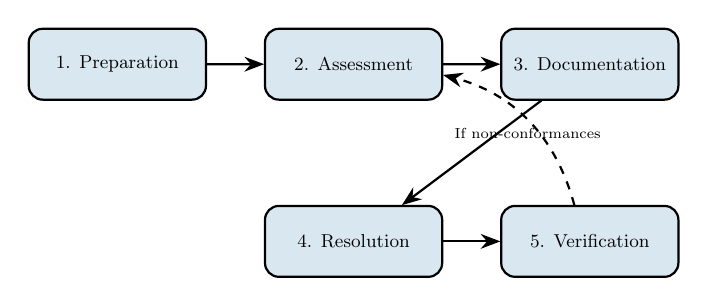
\begin{tikzpicture}[
    scale=0.75,
    transform shape,
    phase/.style={draw, thick, fill=isocolor!15, minimum width=3cm, minimum height=1.2cm, rounded corners=5pt, font=\small, align=center},
    arrow/.style={-{Stealth[length=2.5mm]}, thick}
]
    \node[phase] (prep) at (0,4) {1. Preparation};
    \node[phase] (assess) at (4,4) {2. Assessment};
    \node[phase] (doc) at (8,4) {3. Documentation};
    \node[phase] (resolve) at (4,1) {4. Resolution};
    \node[phase] (verify) at (8,1) {5. Verification};
    
    \draw[arrow] (prep) -- (assess);
    \draw[arrow] (assess) -- (doc);
    \draw[arrow] (doc) -- (resolve);
    \draw[arrow] (resolve) -- (verify);
    \draw[arrow, dashed] (verify) to[bend right=30] node[below, font=\scriptsize] {If non-conformances} (assess);
\end{tikzpicture}
\caption{Conformance Review Process}
\end{figure}

\subsection{Review Phases}

\begin{longtable}{@{}L{2.5cm} L{5cm} L{5cm}@{}}
\caption{Review Phase Activities} \\
\toprule
\textbf{Phase} & \textbf{Activities} & \textbf{Outputs} \\
\midrule
\endfirsthead
\bottomrule
\endlastfoot
1. Preparation & Gather AD and supporting materials; identify reviewers; schedule review; distribute question sets & Review plan; reviewer assignments; materials distributed \\
2. Assessment & Reviewers complete question sets; identify conformances and gaps; gather evidence & Completed question sets; preliminary findings \\
3. Documentation & Compile findings; classify non-conformances; create assessment report & Conformance assessment report; non-conformance list \\
4. Resolution & Architect addresses non-conformances; updates AD; documents resolutions & Updated AD; resolution documentation \\
5. Verification & Re-assess resolved items; verify conformance; issue final report & Final conformance report; certificate (if applicable) \\
\end{longtable}

\subsection{Review Team Roles}

\begin{longtable}{@{}L{3cm} L{4.5cm} L{5cm}@{}}
\caption{Review Team Roles} \\
\toprule
\textbf{Role} & \textbf{Responsibilities} & \textbf{Qualifications} \\
\midrule
\endfirsthead
\bottomrule
\endlastfoot
Review Lead & Plan and coordinate review; facilitate sessions; compile report & ISO 42010 expertise; review experience \\
Architect & Present AD; answer questions; resolve non-conformances & System and AD knowledge \\
Domain Expert & Assess stakeholder/concern completeness & Domain knowledge; stakeholder perspective \\
Standards Expert & Verify conformance to ISO 42010 requirements & ISO 42010 expertise \\
Recorder & Document findings and decisions & Technical writing skills \\
\end{longtable}

\subsection{Review Session Agenda}

\begin{bestpractice}
\textbf{Typical Conformance Review Session (4-6 hours)}

\textbf{1. Opening (30 min)}
\begin{itemize}[nosep]
    \item Introductions and role assignments
    \item Review objectives and process
    \item Overview of ISO 42010 requirements
\end{itemize}

\textbf{2. AD Presentation (60 min)}
\begin{itemize}[nosep]
    \item Architect presents AD structure and content
    \item Walkthrough of key sections
    \item Questions for clarification
\end{itemize}

\textbf{3. Conformance Assessment (120-180 min)}
\begin{itemize}[nosep]
    \item Systematic review using question sets
    \item Evidence gathering for each requirement
    \item Discussion of findings
\end{itemize}

\textbf{4. Non-Conformance Documentation (30-60 min)}
\begin{itemize}[nosep]
    \item Compile non-conformances
    \item Classify severity
    \item Identify resolution approach
\end{itemize}

\textbf{5. Closing (30 min)}
\begin{itemize}[nosep]
    \item Summarize findings
    \item Agree on next steps
    \item Schedule follow-up if needed
\end{itemize}
\end{bestpractice}

%==============================================================================
\section{Appendix A: Viewpoint Specification Template}
%==============================================================================

\begin{isorequirement}[Viewpoint Specification Template]

\textbf{Viewpoint Name:} [Unique, descriptive name]

\textbf{Viewpoint Overview:} [Brief description of the viewpoint's purpose]

\textbf{Stakeholders Addressed:}
\begin{itemize}[nosep]
    \item [Stakeholder 1]
    \item [Stakeholder 2]
\end{itemize}

\textbf{Concerns Framed:}
\begin{itemize}[nosep]
    \item [Concern 1]
    \item [Concern 2]
\end{itemize}

\textbf{Model Kinds:}

\textit{Model Kind 1:}
\begin{itemize}[nosep]
    \item \textbf{Name:} [Model kind name]
    \item \textbf{Language/Notation:} [e.g., UML Component Diagram]
    \item \textbf{Construction Conventions:} [How to build models]
    \item \textbf{Interpretation Conventions:} [How to read models]
    \item \textbf{Operations:} [Analyses or transformations, if any]
\end{itemize}

\textbf{Source:} [Reference to published viewpoint, if applicable]

\textbf{Correspondence Rules:} [Rules relating this viewpoint to others]
\end{isorequirement}

%==============================================================================
\section{Appendix B: Non-Conformance Report Template}
%==============================================================================

\begin{checklistbox}[Non-Conformance Report]

\textbf{Report ID:} NCR-[number]

\textbf{Date Identified:} [date]

\textbf{AD Reference:} [AD identifier and version]

\textbf{Requirement Reference:} ISO/IEC/IEEE 42010 \S[section]

\textbf{Requirement Text:} [Quote or paraphrase the requirement]

\textbf{Non-Conformance Description:}

[Detailed description of how the AD fails to meet the requirement]

\textbf{Evidence:}

[Specific references to AD sections; what was expected vs. found]

\textbf{Severity:} Critical / Major / Minor

\textbf{Impact:}

[Impact on AD usability, stakeholder needs, or conformance claim]

\textbf{Recommended Resolution:}

[Specific actions to achieve conformance]

\textbf{Resolution Status:} Open / In Progress / Resolved / Verified

\textbf{Resolution Notes:}

[How the non-conformance was resolved; verification evidence]
\end{checklistbox}

%==============================================================================
\section{Appendix C: Glossary}
%==============================================================================

\begin{description}[leftmargin=3cm, style=nextline]
    \item[Architecture] Fundamental concepts or properties of a system embodied in its elements, relationships, and principles of design and evolution
    \item[Architecture Description] Work product used to express an architecture
    \item[Architecture Framework] Conventions, principles, and practices for architecture description in a specific domain
    \item[Concern] Interest in a system relevant to one or more stakeholders
    \item[Conformance] Fulfillment of specified requirements
    \item[Correspondence] Relation between AD elements expressing architecture relationships
    \item[Correspondence Rule] Rule governing correspondences; defines constraints on AD elements
    \item[Model] Artifact expressing information from a perspective defined by a model kind
    \item[Model Kind] Conventions for a type of modeling
    \item[Stakeholder] Individual, team, or organization with interest in a system
    \item[View] Work product expressing architecture from perspective of specific concerns
    \item[Viewpoint] Conventions for constructing, interpreting, and using views
\end{description}

%==============================================================================
\section{Appendix D: References}
%==============================================================================

\begin{enumerate}
    \item ISO/IEC/IEEE 42010:2011. \textit{Systems and software engineering---Architecture description}.
    
    \item ISO/IEC/IEEE 42020:2019. \textit{Software, systems and enterprise---Architecture processes}.
    
    \item ISO/IEC/IEEE 42030:2019. \textit{Software, systems and enterprise---Architecture evaluation framework}.
    
    \item Clements, P., et al. (2010). \textit{Documenting Software Architectures: Views and Beyond} (2nd ed.). Addison-Wesley.
    
    \item Rozanski, N., \& Woods, E. (2011). \textit{Software Systems Architecture} (2nd ed.). Addison-Wesley.
    
    \item Hilliard, R. (2011). ``ISO/IEC/IEEE 42010---The New Standard for Architecture Description.'' \textit{IEEE Software}, 28(3).
    
    \item The Open Group. (2018). \textit{TOGAF Standard, Version 9.2}. Van Haren Publishing.
    
    \item Kruchten, P. (1995). ``The 4+1 View Model of Architecture.'' \textit{IEEE Software}, 12(6), 42-50.
\end{enumerate}

\end{document}